\documentclass[a4paper,11pt]{article}

% ============================================================
%  Le Collé — Séance 1 : Déterminants, courbes paramétrées
%  © 2026 Ahmed Amine Ouqlani
% ============================================================

% ---------- Polices ----------
\usepackage[utf8]{inputenc}
\usepackage[T1]{fontenc}
\usepackage[sc]{mathpazo}          % texte et mathématiques : Palatino
\usepackage[scaled=0.88]{helvet}   % titres et repères : linéale
\linespread{1.07}
\usepackage{amsmath,amssymb,amsthm,mathrsfs,stmaryrd}
\usepackage{microtype}

% ---------- Mise en page ----------
\usepackage[a4paper,top=2.3cm,bottom=2.3cm,left=2.4cm,right=2.4cm,
            headheight=14pt,headsep=0.8cm,footskip=1.1cm]{geometry}
\setlength{\parindent}{0pt}
\setlength{\parskip}{0.45em plus 0.15em minus 0.1em}
\raggedbottom
\emergencystretch=1.5em
\clubpenalty=10000 \widowpenalty=10000 \displaywidowpenalty=10000 \brokenpenalty=10000

% ---------- Couleurs : un bleu de nuit, un ocre, des gris ----------
\usepackage{xcolor}
\definecolor{Ink}{HTML}{1C2533}
\definecolor{Bleu}{HTML}{1F3A5F}
\definecolor{BleuMoyen}{HTML}{4A6A8F}
\definecolor{BleuClair}{HTML}{9DB2C9}
\definecolor{Fond}{HTML}{F2F4F7}
\definecolor{Ocre}{HTML}{B07A26}
\definecolor{Brique}{HTML}{A23B2A}
\definecolor{Gris}{HTML}{5E6672}
\definecolor{Filet}{HTML}{C5CCD6}

% ---------- Packages ----------
\usepackage{enumitem}
\setlist{itemsep=0.25em,topsep=0.35em,parsep=0pt}
\setlist[itemize]{label=\textcolor{BleuMoyen}{\small\textbullet},leftmargin=1.4em}
\setlist[enumerate]{leftmargin=1.8em,label=\textsf{\small\color{Bleu}\arabic*.}}
\usepackage{booktabs,array,multicol}
\usepackage{needspace,float}
\usepackage[font=small,labelfont={sf,color=Bleu},labelsep=period,skip=6pt]{caption}
\usepackage{tikz}
\usetikzlibrary{arrows.meta,calc,decorations.markings}
\usepackage{pgfplots}
\pgfplotsset{compat=1.17}
\usepackage{tkz-tab}
\usepackage[most]{tcolorbox}
\usepackage{titlesec,titletoc}
\usepackage{fancyhdr,lastpage,etoolbox}
\usepackage[colorlinks=true,linkcolor=Bleu,urlcolor=Bleu,citecolor=Bleu,
            pdftitle={Le Collé — TD Propriétés métriques des courbes (corrections)},pdfauthor={Ahmed Amine Ouqlani}]{hyperref}

\numberwithin{equation}{section}
\numberwithin{figure}{section}
\numberwithin{table}{section}

% ---------- Titres ----------
% Chapitres (sections) : grand numéro, titre en linéale, filet ocre
\titleformat{\section}[display]
  {\normalfont\sffamily\color{Ink}}
  {{\small\color{Gris}\textls[200]{\MakeUppercase{Chapitre}}}\\[-0.2em]%
   {\fontsize{64}{64}\selectfont\color{BleuClair}\thesection}}
  {0.4em}
  {\fontsize{25}{30}\selectfont\bfseries}
  [\vspace{0.5em}{\color{Ocre}\rule{3.2cm}{1.4pt}}]
\titlespacing*{\section}{0pt}{0pt}{1.6em}
\titleformat{name=\section,numberless}[display]
  {\normalfont\sffamily\color{Ink}}{}{0pt}{\fontsize{25}{30}\selectfont\bfseries}
  [\vspace{0.5em}{\color{Ocre}\rule{3.2cm}{1.4pt}}]
\titlespacing*{name=\section,numberless}{0pt}{0pt}{1.6em}

\titleformat{\subsection}
  {\needspace{5\baselineskip}\normalfont\sffamily\Large\bfseries\color{Ink}}
  {\color{Bleu}\thesubsection}{0.8em}{}
\titlespacing*{\subsection}{0pt}{1.8em}{0.5em}
\titleformat{\subsubsection}
  {\needspace{5\baselineskip}\normalfont\sffamily\large\bfseries\color{Ink}}
  {\color{Bleu}\thesubsubsection}{0.7em}{}
\titlespacing*{\subsubsection}{0pt}{1.6em}{0.4em}
\titleformat{\paragraph}[runin]{\normalfont\sffamily\bfseries\color{Ink}}{}{0pt}{}[.]
\titlespacing*{\paragraph}{0pt}{0.9em}{0.6em}
\setcounter{secnumdepth}{3}
\setcounter{tocdepth}{2}

% ---------- Table des matières ----------
\titlecontents{section}[0pt]{\addvspace{0.7em}\sffamily\bfseries\color{Ink}}
  {\makebox[2.2em][l]{\color{Bleu}\thecontentslabel}}{}{\hfill\contentspage}[\addvspace{0.2em}]
\titlecontents{subsection}[2.2em]{\small\linespread{1}\selectfont}
  {\makebox[2.6em][l]{\color{Gris}\thecontentslabel}}{}{\titlerule*[0.7pc]{.}\contentspage}

% ---------- En-têtes et pieds de page ----------
\pagestyle{fancy}
\fancyhf{}
\renewcommand{\sectionmark}[1]{\markboth{\thesection\quad#1}{}}
\fancyhead[L]{\footnotesize\sffamily\color{Gris}\leftmark}
\fancyhead[R]{\footnotesize\sffamily\scshape\color{Gris}Le Collé}
\fancyfoot[C]{\small\sffamily\color{Ink}\thepage}
\fancyfoot[L]{\scriptsize\sffamily\hyperlink{toc}{\color{Filet}sommaire}}
\renewcommand{\headrulewidth}{0.4pt}
\renewcommand{\headrule}{{\color{Filet}\hrule height\headrulewidth width\headwidth}}
\renewcommand{\footrulewidth}{0pt}
\fancypagestyle{plain}{\fancyhf{}\fancyfoot[C]{\small\sffamily\color{Ink}\thepage}\renewcommand{\headrulewidth}{0pt}}

% ---------- Énoncés ----------
\newtheoremstyle{enonce}{0pt}{0pt}{}{}{\sffamily\bfseries\color{Bleu}}{.}{0.5em}
  {\thmname{#1}\thmnumber{~#2}\thmnote{\ \normalfont\sffamily\color{Ink}(#3)}}
\newtheoremstyle{exemple}{0.9em}{0.9em}{}{}{\sffamily\bfseries\color{BleuMoyen}}{.}{0.5em}
  {\thmname{#1}\thmnumber{~#2}\thmnote{\ \normalfont\sffamily\color{Ink}(#3)}}
\newtheoremstyle{remarque}{0.7em}{0.7em}{}{}{\sffamily\itshape}{.}{0.5em}{\thmname{#1}\thmnote{\ (#3)}}
\theoremstyle{enonce}
\newtheorem{definition}{Définition}[section]
\newtheorem{theoreme}[definition]{Théorème}
\newtheorem{proposition}[definition]{Proposition}
\newtheorem{corollaire}[definition]{Corollaire}
\theoremstyle{exemple}
\newtheorem{exemple}[definition]{Exemple}
\theoremstyle{remarque}
\newtheorem*{remarque}{Remarque}

\tcbset{
  defi/.style={enhanced,breakable,colback=white,colframe=white,boxrule=0pt,arc=0pt,
     borderline west={1.2pt}{0pt}{Bleu},left=11pt,right=4pt,top=3pt,bottom=3pt,
     before skip=1.1em,after skip=1.1em},
  thm/.style={enhanced,breakable,colback=Fond,colframe=Fond,boxrule=0pt,arc=0pt,
     borderline west={2.4pt}{0pt}{Bleu},left=11pt,right=8pt,top=6pt,bottom=6pt,
     before skip=1.2em,after skip=1.2em}}
\tcolorboxenvironment{definition}{defi}
\tcolorboxenvironment{theoreme}{thm}
\tcolorboxenvironment{proposition}{thm}
\tcolorboxenvironment{corollaire}{thm}

\renewcommand{\proofname}{Démonstration}
\renewcommand{\qedsymbol}{\textcolor{BleuClair}{$\blacksquare$}}
\makeatletter
\renewenvironment{proof}[1][\proofname]{\par\pushQED{\qed}\normalfont
  \topsep0.5em\relax\trivlist\item[\hskip\labelsep\sffamily\itshape\color{Gris}#1.]\ignorespaces}
  {\popQED\endtrivlist\@endpefalse}
\makeatother

% ---------- Méthode : filets haut et bas, titre en bandeau ----------
\makeatletter\newcommand{\methlabelfix}{\protected@edef\@currentlabel{\thetcbcounter}}\makeatother
\newtcolorbox[auto counter,number within=section]{methode}[2][]{%
  enhanced,unbreakable,colback=white,colframe=white,boxrule=0pt,arc=0pt,
  borderline north={0.9pt}{0pt}{Bleu},borderline south={0.9pt}{0pt}{Bleu},
  left=4pt,right=4pt,top=8pt,bottom=8pt,before skip=1.4em,after skip=1.4em,
  before upper={\methlabelfix\phantomsection\addcontentsline{met}{metentry}{\protect\makebox[2.6em][l]{\thetcbcounter}#2}%
     {\sffamily\bfseries\small\color{white}\colorbox{Bleu}{\strut\ MÉTHODE~\thetcbcounter\ }}%
     \ \ {\sffamily\bfseries\color{Bleu}#2}\par\smallskip},#1}

% ---------- Repères pédagogiques : un filet de couleur, un mot-clé ----------
\newcommand{\definirbloc}[3]{% nom, couleur, libellé
  \newtcolorbox{#1}[1][]{enhanced,breakable,blanker,
    borderline west={1.4pt}{0pt}{#2},left=10pt,right=2pt,top=1pt,bottom=1pt,
    before skip=1em,after skip=1em,
    before upper={{\sffamily\bfseries\footnotesize\color{#2}\textls[120]{\MakeUppercase{#3}}}\quad},##1}}
\definirbloc{reflexe}{Bleu}{Réflexe}
\definirbloc{astuce}{Ocre}{Astuce}
\definirbloc{attention}{Brique}{Attention}
\definirbloc{enpratique}{BleuMoyen}{En pratique}
\definirbloc{plusloin}{Gris}{Pour aller plus loin}
\definirbloc{strategie}{Bleu}{Stratégie}
\definirbloc{lecture}{BleuMoyen}{Lire le schéma}
% compatibilité avec les parties reprises
\newenvironment{garde}{\begin{attention}}{\end{attention}}
\newenvironment{complementHP}{\begin{plusloin}}{\end{plusloin}}
\newenvironment{interpretation}{\begin{enpratique}}{\end{enpratique}}

% ---------- Exercices, corrigés ----------
\newcounter{exo}[section]
\renewcommand{\theexo}{\thesection.\arabic{exo}}
\newcommand{\niveau}[1]{{\color{Ocre}\footnotesize
  \ifcase#1\or$\bullet\circ\circ\circ\circ$\or$\bullet\bullet\circ\circ\circ$\or$\bullet\bullet\bullet\circ\circ$%
  \or$\bullet\bullet\bullet\bullet\circ$\or$\bullet\bullet\bullet\bullet\bullet$\fi}}
\newcommand{\serie}[1]{\par\needspace{8\baselineskip}\vspace{1.5em}%
  \noindent{\sffamily\bfseries\color{Bleu}#1}\par\nobreak\vspace{-0.4em}%
  \noindent{\color{Filet}\rule{\linewidth}{0.4pt}}\par\nobreak\vspace{0.1em}}
\newenvironment{exo}[3]{%
  \par\needspace{5\baselineskip}\vspace{0.75em}\refstepcounter{exo}\label{e:#1}%
  \def\exolab{#1}%
  \noindent{\sffamily\bfseries\color{Bleu}Exercice~\theexo}\quad\niveau{#2}%
  \hfill{\footnotesize\sffamily\color{Gris}#3}\par\nobreak\vspace{0.15em}}%
  {\par\nopagebreak\noindent\hfill{\scriptsize\sffamily\hyperref[c:\exolab]{\color{Gris}corrigé p.~\pageref{c:\exolab}}}\par}
\newenvironment{corrige}[1]{%
  \par\needspace{6\baselineskip}\vspace{1em}\phantomsection\label{c:#1}%
  \noindent{\sffamily\bfseries\color{Bleu}Exercice~\ref{e:#1}}\quad
  {\scriptsize\sffamily\hyperref[e:#1]{\color{Gris}énoncé p.~\pageref{e:#1}}}\par\nobreak\vspace{0.2em}}%
  {\hfill\textcolor{BleuClair}{$\square$}\par}
\newcommand{\etape}[1]{\par\smallskip\noindent{\sffamily\bfseries\small\color{BleuMoyen}#1.}\ }
\newenvironment{solution}{\par\noindent{\sffamily\bfseries\small\color{BleuMoyen}Solution.}\ }{\hfill\textcolor{BleuClair}{$\square$}\par}
\newcommand{\chercher}{\par\smallskip\noindent{\color{Filet}\rule[0.5ex]{1.2cm}{0.4pt}}\
  {\footnotesize\sffamily\itshape\color{Gris}laisser chercher l'étudiant avant de poursuivre}\par\smallskip}

% ---------- Guide de séance ----------

\newcommand{\marge}[1]{\leavevmode\marginpar{\raggedleft\scriptsize\sffamily\color{Gris}\textls[100]{\MakeUppercase{#1}}}\ignorespaces}
\newcommand{\Etape}[4]{%
  \subsection[Étape #1 --- #3 {\color{Gris}(#2)}]{#3}\label{etape:#1}%
  \noindent{\small\sffamily\color{Gris}{\color{Ocre}\bfseries Étape #1}\quad·\quad #2\quad·\quad #4}\par\medskip}
\newcommand{\question}[1]{\par\smallskip\noindent{\sffamily\bfseries\small\color{BleuMoyen}Question.}\ \textit{#1}\par\smallskip}
\newcommand{\rappel}[1]{\par\smallskip\noindent\phantomsection\addcontentsline{rap}{rapentry}{#1}%
  {\sffamily\bfseries\scriptsize\colorbox{Fond}{\color{Gris}\strut RAPPEL}}\ {\sffamily\small\color{Gris}#1.}\ }
\newcommand{\pourquoi}{\par\noindent{\sffamily\bfseries\small\color{Ocre}Pourquoi ?}\ }

% Ouverture de chapitre : \ouverture{objectifs}{prérequis}{durée}
\newcommand{\ouverture}[3]{%
  \begin{tcolorbox}[enhanced,colback=Fond,colframe=Fond,arc=0pt,boxrule=0pt,left=12pt,right=12pt,top=10pt,bottom=10pt,
     before skip=1.2em,after skip=1.6em]
  \begin{minipage}[t]{0.56\linewidth}
  {\sffamily\bfseries\small\color{Bleu}OBJECTIFS}\par\vspace{0.3em}\small #1
  \end{minipage}\hfill
  \begin{minipage}[t]{0.38\linewidth}
  {\sffamily\bfseries\small\color{Bleu}PRÉREQUIS}\par\vspace{0.3em}\small #2
  \ifx\relax#3\relax\else\par\vspace{0.6em}{\sffamily\bfseries\small\color{Bleu}DURÉE}\par\vspace{0.2em}\small #3\fi
  \end{minipage}
  \end{tcolorbox}}
% Fin de chapitre
\newenvironment{essentiel}{\par\needspace{12\baselineskip}\vspace{1.5em}%
  \begin{tcolorbox}[enhanced,unbreakable,colback=white,colframe=white,boxrule=0pt,arc=0pt,
   borderline north={1.4pt}{0pt}{Ocre},left=2pt,right=2pt,top=8pt,bottom=4pt]
  {\sffamily\bfseries\color{Ocre}L'ESSENTIEL DU CHAPITRE}\par\medskip}{\end{tcolorbox}}

% ---------- Notations ----------
\newcommand{\K}{\mathbb{K}}
\newcommand{\R}{\mathbb{R}}
\newcommand{\C}{\mathbb{C}}
\newcommand{\N}{\mathbb{N}}
\newcommand{\Z}{\mathbb{Z}}
\newcommand{\Mn}[1]{\mathcal{M}_{n}(#1)}
\newcommand{\GLn}[1]{\mathrm{GL}_n(#1)}
\newcommand{\LE}{\mathcal{L}(E)}
\newcommand{\rg}{\operatorname{rg}}
\newcommand{\vect}{\operatorname{Vect}}
\newcommand{\Mat}{\operatorname{Mat}}
\newcommand{\Id}{\operatorname{Id}}
\newcommand{\sh}{\operatorname{sh}}
\newcommand{\ch}{\operatorname{ch}}
\renewcommand{\th}{\operatorname{th}}
\DeclareMathOperator{\argsh}{argsh}
\newcommand{\vv}[1]{\overrightarrow{#1}}
\newcommand{\ve}[1]{\vec{#1}}
\newcommand{\ient}[2]{\llbracket #1,#2\rrbracket}
\newcommand{\dt}[1]{\left|\begin{matrix}#1\end{matrix}\right|}
\newcommand{\dis}{\displaystyle}

% ---------- Figures ----------
\pgfplotsset{trig format plots=rad}
\pgfplotsset{courbe/.style={axis lines=middle,axis equal image,
  axis line style={Gris,-{Stealth[length=5pt]}},
  xlabel={$x$},ylabel={$y$},ticklabel style={font=\scriptsize\sffamily,color=Gris},
  every axis x label/.style={at={(ticklabel* cs:1)},anchor=west,font=\small},
  every axis y label/.style={at={(ticklabel* cs:1)},anchor=south,font=\small},
  samples=300,smooth,width=0.6\linewidth}}
\tikzset{arcetude/.style={Bleu,line width=1.25pt},
         reste/.style={BleuClair,line width=1pt},
         tgte/.style={Ocre,line width=0.9pt},
         asy/.style={Gris,dashed,line width=0.6pt},
         pt/.style={circle,fill=Ink,inner sep=1.2pt}}

% ---------- Navigation ----------
\makeatletter
\newcommand*\l@rapentry{\@dottedtocline{1}{0em}{0em}}
\newcommand*\l@metentry{\@dottedtocline{1}{0em}{0em}}
\newcommand{\listemethodes}{\@starttoc{met}}
\newcommand{\listerappels}{\@starttoc{rap}}
\makeatother
% onglets de chapitre sur le bord droit
\usepackage{eso-pic}
\newif\ifonglets \ongletsfalse
\newcommand{\dessineronglet}{%
  \edef\ongcol{\ifnum\value{section}=3 Ocre\else Bleu\fi}%
  \edef\ongnum{\the\value{section}}%
  \pgfmathsetmacro{\ongy}{3.2+2.3*(\ongnum-1)}%
  \begin{tikzpicture}[remember picture,overlay]
  \fill[\ongcol] ([xshift=-0.75cm,yshift=-\ongy cm]current page.north east)
     rectangle ([yshift=-\ongy cm-1.9cm]current page.north east);
  \node[text=white,font=\sffamily\bfseries\large] at ([xshift=-0.37cm,yshift=-\ongy cm-0.95cm]current page.north east)
     {\ongnum};
  \end{tikzpicture}}
\AddToShipoutPictureBG{\ifonglets\ifnum\value{section}>0 \dessineronglet\fi\fi}
% blocs de navigation et d'enseignement
\definirbloc{commencer}{Gris}{Si vous commencez ici}
\definirbloc{horsprogramme}{Brique}{Hors programme}
\newcommand{\HP}{\,{\sffamily\bfseries\scriptsize\textcolor{Brique}{[HP]}}}
\newcommand{\source}[1]{{\footnotesize\sffamily\color{Gris}\,(#1)}}
\newcommand{\coupdepouce}[1]{\par\vspace{-0.2em}\noindent{\footnotesize\sffamily\color{Gris}%
  \textbf{Coup de pouce} (à donner si l'étudiant bloque) : #1}\par}
\newcommand{\pointarret}[1]{\par\vspace{1em}\noindent{\color{Filet}\rule[0.5ex]{\linewidth}{0.4pt}}\par\nobreak
  \noindent{\footnotesize\sffamily\color{Ocre}\bfseries POINT D'ARRÊT POSSIBLE}\quad{\footnotesize\sffamily\color{Gris}#1}\par\vspace{0.6em}}
\newcommand{\demarche}[1]{\noindent{\sffamily\bfseries\small\color{BleuMoyen}Démarche.}\ \textit{#1}\par\smallskip}

% ---------- Corrigés : idées, astuces, pièges, à retenir ----------
\newcommand{\choix}[1]{\par\noindent{\sffamily\bfseries\small\color{BleuMoyen}Choix de la méthode.}\ #1\par\smallskip}
\newcommand{\gain}[1]{\par\noindent{\sffamily\bfseries\small\color{Ocre}Astuce.}\ #1\par}
\newcommand{\piege}[1]{\par\noindent{\sffamily\bfseries\small\color{Brique}Piège.}\ #1\par}
\newtcolorbox{retenirbox}{enhanced,breakable,colback=Fond,colframe=Fond,arc=0pt,boxrule=0pt,
  borderline west={2pt}{0pt}{Ocre},left=8pt,right=6pt,top=4pt,bottom=4pt,before skip=0.7em,after skip=0.5em}
\newcommand{\retenir}[1]{\begin{retenirbox}{\sffamily\bfseries\footnotesize\color{Ocre}À RETENIR}\quad #1\end{retenirbox}}
\newcommand{\TD}[1]{{\color{Ocre}\bfseries TD\,#1}\ ·\ }
\newcommand{\q}[1]{\par\smallskip\noindent{\sffamily\bfseries\color{Bleu}#1}\ }
\providecommand{\iddots}{\mathinner{\mkern1mu\raise1pt\hbox{.}\mkern2mu\raise4pt\hbox{.}\mkern2mu\raise7pt\hbox{.}\mkern1mu}}


% ================================================================ TD : mise en page propre au livret d'exercices
\fancyhf{}
\fancyhead[L]{\footnotesize\sffamily\color{Gris}TD · Propriétés métriques des courbes · corrections}
\fancyhead[R]{\footnotesize\sffamily\scshape\color{Gris}Le Collé}
\fancyfoot[C]{\small\sffamily\color{Ink}\thepage\,/\,\pageref{LastPage}}
\fancypagestyle{plain}{\fancyhf{}\fancyfoot[C]{\small\sffamily\color{Ink}\thepage\,/\,\pageref{LastPage}}\renewcommand{\headrulewidth}{0pt}}
\makeatletter
\newcommand{\partie}[3]{% numéro, titre, description
  \par\needspace{10\baselineskip}\vspace{1.4em}\phantomsection\label{partie:#1}\pdfbookmark[0]{Partie #1}{partie.#1}%
  {\sffamily\small\color{Gris}\textls[200]{PARTIE #1}}\par\nobreak\vspace{0.1em}
  {\sffamily\bfseries\LARGE\color{Ink}#2}\par\nobreak\vspace{0.3em}
  {\color{Ocre}\rule{2.6cm}{1.2pt}}\par\nobreak\vspace{0.2em}
  {\small\color{Gris}#3}\par\nobreak\vspace{0.6em}}
\newcommand{\exercice}[7]{% numéro, difficulté, titre, origine, notions, identifiant, page du corrigé
  \par\needspace{8\baselineskip}\vspace{1.1em}\phantomsection
  \def\@currentlabel{#1}\label{e:#6}\pdfbookmark[1]{Exercice #1}{e.#6}%
  \noindent{\sffamily\bfseries\large\color{Bleu}Exercice~#1}\quad\niveau{#2}\hfill{\footnotesize\sffamily\color{Gris}#4}\par\nobreak
  \vspace{0.1em}\noindent{\sffamily\bfseries\color{Ink}#3}\par\nobreak
  \vspace{0.1em}\noindent{\footnotesize\sffamily\color{Gris}Notions : #5.\hfill\mbox{corrigé p.~#7}\par}\nobreak
  \vspace{0.35em}}
\newcommand{\renvoi}[1]{\par\nopagebreak\vspace{0.2em}\noindent\hfill{\scriptsize\sffamily\color{Gris}#1}\par}
\newcommand{\place}{\par\vspace{1.6cm plus 0.6cm minus 0.6cm}}
\newcommand{\correction}[4]{% numéro, titre, identifiant, renvoi
  \par\needspace{7\baselineskip}\vspace{1.3em}\phantomsection
  \def\@currentlabel{#1}\label{e:#3}\pdfbookmark[1]{Exercice #1}{c.#3}%
  {\color{Filet}\hrule height 0.4pt}\vspace{0.5em}
  \noindent{\sffamily\bfseries\large\color{Bleu}Exercice~#1}\quad{\sffamily\bfseries\color{Ink}#2}\hfill{\scriptsize\sffamily\color{Gris}#4}\par\nobreak
  \vspace{0.4em}}
\newcommand{\sommaireligne}[3]{\noindent\hbox to 2.2em{\hfill\sffamily\color{Bleu}#1.}\enspace\begin{minipage}[t]{0.8\linewidth}\raggedright#2\end{minipage}\hfill\pageref{e:#3}\par}
\makeatother
\setlength{\parskip}{0.5em plus 0.15em minus 0.1em}

\begin{document}
\thispagestyle{plain}
{\sffamily\small\color{Gris}\textls[150]{LE COLLÉ · MATHÉMATIQUES PT · CHAPITRE 3}}\par\vspace{0.2em}
{\sffamily\bfseries\fontsize{26}{30}\selectfont\color{Ink}TD --- Propriétés métriques des courbes}\par\vspace{0.3em}
{\sffamily\Large\color{BleuMoyen}Corrections}\par\vspace{0.4em}
{\color{Ocre}\rule{3.2cm}{1.4pt}}\par\vspace{0.8em}
{\small Corrections détaillées des 24 exercices du TD, dans le même ordre et avec les mêmes numéros.
Chaque correction commence par le choix de la méthode, puis détaille les calculs ; les encadrés « À retenir » résument ce qui
resservira. Les renvois « méthode~1.4 du livre », « théorème~2.3 du volume~2 »… désignent le cours.
\textbf{Chercher d'abord l'exercice} avant d'ouvrir sa correction.}

\partie{I}{Applications directes du cours}{}
\correction{1}{Courbure d'un cercle, d'une droite}{met-cercle}{énoncé : TD, p.~2}
\q{1.} $f'(t)=r(-\sin t,\cos t)$, $\|f'\|=r$, donc $s=rt$. $\ve T=(-\sin t,\cos t)$, $\ve N=(-\cos t,-\sin t)$ : la normale est dirigée vers le centre $\Omega(a,b)$. $f''=-r(\cos t,\sin t)$ et $\det(f',f'')=r^2(\sin^2t+\cos^2t)=r^2$, d'où $\gamma=\frac{r^2}{r^3}=\frac1r$, $R=r$ et $I=M+r\ve N=\Omega$ : le cercle est son propre cercle de courbure ; sa développée est réduite au point $\Omega$.

\q{2.} $f'=\ve u$, $f''=\ve0$ : $\gamma=0$ en tout point. La courbure est nulle, il n'y a pas de centre de courbure (on dit parfois « rayon infini »).
\retenir{courbure constante $\frac1r$ pour un cercle de rayon $r$ parcouru dans le sens direct (elle vaut $-\frac1r$ dans le sens indirect) ; nulle pour une droite.}
\par\hfill\textcolor{BleuClair}{$\square$}\par
\correction{2}{Longueur de la cardioïde}{ex-cardio}{énoncé : TD, p.~2}
\q{1.} $x'=\sin t\cos t-(1-\cos t)\sin t=\sin2t-\sin t$ et $y'=\sin^2t+(1-\cos t)\cos t=\cos t-\cos2t$. Donc
\[x'^2+y'^2=(\sin^2 2t+\cos^2 2t)+(\sin^2t+\cos^2t)-2(\sin2t\sin t+\cos2t\cos t),\]
c'est-à-dire $x'^2+y'^2=2-2\cos t=4\sin^2\frac t2$.

\q{2.} Sur $[0,2\pi]$, $\sin\frac t2\geq0$, donc $\|f'(t)\|=2\sin\frac t2$ (sans valeur absolue) et
\[L=\int_0^{2\pi}2\sin\tfrac t2\,dt=\left[-4\cos\tfrac t2\right]_0^{2\pi}=8.\]

\q{3.} On trouverait $16$ : la courbe est parcourue deux fois. Une longueur mesure le chemin \emph{parcouru} ; on intègre sur un intervalle où chaque arc n'est décrit qu'une fois.
\piege{oublier la valeur absolue : $\sqrt{4\sin^2\frac t2}=2\left|\sin\frac t2\right|$.}
\par\hfill\textcolor{BleuClair}{$\square$}\par
\correction{3}{Longueur d'une arche de cycloïde}{m-cycl}{énoncé : TD, p.~2}
\choix{on calcule $\|f'\|$ en factorisant par l'angle moitié, pour que la racine carrée tombe exactement.}
$f'(t)=(1-\cos t,\sin t)=\left(2\sin^2\tfrac t2,\ 2\sin\tfrac t2\cos\tfrac t2\right)=2\sin\tfrac t2\left(\sin\tfrac t2,\cos\tfrac t2\right)$,
d'où $\|f'(t)\|=2\left|\sin\frac t2\right|=2\sin\frac t2$ sur $[0,2\pi]$.

\q{1.} $L=\int_0^{2\pi}2\sin\frac t2\,dt=\left[-4\cos\frac t2\right]_0^{2\pi}=8$.

\q{2.} $s(t)=\int_0^t2\sin\frac u2\,du=4\left(1-\cos\frac t2\right)$ pour $t\in[0,2\pi]$.
\gain{l'écriture $f'=v(\cos\alpha,\sin\alpha)$ obtenue ici sert aussi pour la courbure : on lit $v=2\sin\frac t2$ et
$\alpha=\frac\pi2-\frac t2$ (exercice~\ref{e:m-cycl-dev}).}
\piege{$\sqrt{4\sin^2\frac t2}=2|\sin\frac t2|$ : sur $[2\pi,4\pi]$, le sinus est négatif ; sans valeur absolue, la deuxième arche
aurait une « longueur » $-8$.}
\retenir{$\sqrt{x'^2+y'^2}$ devient simple quand $1-\cos t=2\sin^2\frac t2$ et $\sin t=2\sin\frac t2\cos\frac t2$ s'appliquent.}
\par\hfill\textcolor{BleuClair}{$\square$}\par
\correction{4}{Longueur sur la chaînette}{met-chain}{énoncé : TD, p.~3}
$f(x)=(x,\ch x)$, $\|f'\|=\sqrt{1+\sh^2x}=\ch x$ (positif). Donc $L=\int_0^a\ch x\,dx=\sh a$. L'abscisse curviligne d'origine $A$, orientée dans le sens des $x$ croissants, est $s(x)=\sh x$ (valable pour tout $x\in\R$).
\par\hfill\textcolor{BleuClair}{$\square$}\par
\correction{5}{Longueur d'un arc de parabole}{met-parab}{énoncé : TD, p.~3}
On paramètre par $f(x)=\left(x,\frac{x^2}2\right)$ : $\|f'(x)\|=\sqrt{1+x^2}$ et $L=\int_0^1\sqrt{1+x^2}\,dx$.
On pose $x=\sh u$, $dx=\ch u\,du$, $\sqrt{1+x^2}=\ch u$ :
\[L=\int_0^{\argsh1}\ch^2u\,du=\left[\frac u2+\frac{\sh2u}4\right]_0^{\argsh1}=\left[\frac u2+\frac{\sh u\ch u}2\right]_0^{\argsh1}.\]
Avec $\argsh1=\ln(1+\sqrt2)$, $\sh u=1$ et $\ch u=\sqrt2$ : $L=\dfrac{\sqrt2+\ln(1+\sqrt2)}2\approx1{,}148$.
\gain{pour $\sqrt{1+x^2}$, le changement $x=\sh u$ fait disparaître la racine ; pour $\sqrt{1-x^2}$, c'est $x=\sin u$.}
\par\hfill\textcolor{BleuClair}{$\square$}\par
\correction{6}{Courbure d'un graphe}{met-graphe}{énoncé : TD, p.~3}
\q{1.} $f'=(1,g')$, $f''=(0,g'')$, $\det(f',f'')=g''$ et $\|f'\|=\sqrt{1+g'^2}$, d'où $\gamma=\frac{\det(f',f'')}{\|f'\|^3}=\frac{g''}{(1+g'^2)^{3/2}}$.

\q{2.} Pour $g(x)=x^2$ : $g'(0)=0$, $g''(0)=2$, $\gamma(0)=2$, $R=\frac12$. Pour $g=\ln$ : $g'(1)=1$, $g''(1)=-1$, $\gamma(1)=\frac{-1}{2^{3/2}}$, donc $|R|=2\sqrt2$ (le signe négatif indique que la courbe tourne dans le sens indirect, vers sa droite).
\par\hfill\textcolor{BleuClair}{$\square$}\par
\correction{7}{Cercle de courbure d'un graphe}{met-osc-exp}{énoncé : TD, p.~3}
\q{1.} Avec $g=\exp$ : $g'(0)=g''(0)=1$, donc $\gamma(0)=\dfrac{1}{(1+1)^{3/2}}=\dfrac1{2\sqrt2}$ et $R=2\sqrt2$.

\q{2.} $f(x)=(x,e^x)$, $f'(0)=(1,1)$, $\ve T=\frac1{\sqrt2}(1,1)$ et $\ve N=\frac1{\sqrt2}(-1,1)$. Donc
\[I=A+R\ve N=(0,1)+2\sqrt2\cdot\tfrac1{\sqrt2}(-1,1)=(-2,3).\]
Le cercle de courbure a pour équation $(x+2)^2+(y-3)^2=8$ ; il passe bien par $A$ ($4+4=8$) et il est tangent en $A$ à la courbe (son centre est sur la normale).
\retenir{le centre de courbure est sur la normale, du côté où la courbe tourne ($\gamma>0$ : du côté de $\ve N$).}
\par\hfill\textcolor{BleuClair}{$\square$}\par
\correction{8}{Une première enveloppe}{met-env-cercle}{énoncé : TD, p.~4}
On résout le système formé de l'équation et de sa dérivée par rapport à $t$ :
\[\begin{cases}x\cos t+y\sin t=1\\-x\sin t+y\cos t=0\end{cases}\]
de déterminant $1$ : $x=\cos t$, $y=\sin t$. L'enveloppe est le cercle unité ; $\mathcal D_t$ est sa tangente au point $(\cos t,\sin t)$ (elle est orthogonale au rayon et à distance $1$ de $O$).
\par\hfill\textcolor{BleuClair}{$\square$}\par
\correction{9}{Une parabole comme enveloppe}{met-env-parab}{énoncé : TD, p.~4}
\q{1.} L'équation $\frac xt+\frac y{1-t}=1$ (droite qui coupe les axes en $P$ et $Q$), multipliée par $t(1-t)$, donne $(1-t)x+ty=t(1-t)$.

\q{2.} On dérive par rapport à $t$, $x$ et $y$ fixés : $-x+y=1-2t$. Le système
\[\begin{cases}(1-t)x+ty=t-t^2\\-x+y=1-2t\end{cases}\]
a pour déterminant $(1-t)+t=1$. La seconde équation donne $y=x+1-2t$ ; en reportant : $x+t(1-2t)=t-t^2$, d'où $x=t^2$, puis $y=(1-t)^2$. L'enveloppe est $t\mapsto\big(t^2,(1-t)^2\big)$, $t\in\,]0,1[$, et $\sqrt x+\sqrt y=t+(1-t)=1$.

\q{3.} $x-y=2t-1$ et $x+y=2t^2-2t+1$, donc $(x-y)^2-2(x+y)+1=4t^2-4t+1-4t^2+4t-2+1=0$. La partie quadratique $(x-y)^2$ est un carré : c'est une parabole (d'axe dirigé par $(1,1)$), tangente aux axes en $(1,0)$ et $(0,1)$.
\gain{le point de contact $\big(t^2,(1-t)^2\big)$ est sur le segment $[PQ]$ : c'est $P+(1-t)\vv{PQ}$.}
\par\hfill\textcolor{BleuClair}{$\square$}\par
\partie{II}{Exercices classiques et méthodes incontournables}{}
\correction{10}{Longueur totale de l'astroïde}{m-astro}{énoncé : TD, p.~5}
\choix{la courbe a quatre arcs symétriques ; on calcule la longueur d'un arc, où $\|f'\|$ s'écrit sans valeur absolue.}
$f'(t)=3\sin t\cos t\,(-\cos t,\sin t)$, donc $\|f'(t)\|=3|\sin t\cos t|$. Sur $\left[0,\frac\pi2\right]$, $\sin t\cos t\geq0$ :
\[L=4\int_0^{\pi/2}3\sin t\cos t\,dt=4\times\frac32\left[\sin^2t\right]_0^{\pi/2}=6.\]
\piege{$\int_0^{2\pi}3\sin t\cos t\,dt=0$ : oublier la valeur absolue donne une longueur nulle. Les quatre points stationnaires
(rebroussements) ne gênent pas le calcul : on intègre sur chaque arc régulier.}
\retenir{longueur totale = nombre d'arcs symétriques $\times$ longueur d'un arc, sur lequel le signe de $\|f'\|$ est connu.}
\par\hfill\textcolor{BleuClair}{$\square$}\par
\correction{11}{Courbure de l'ellipse aux sommets}{m-ellipse}{énoncé : TD, p.~5}
\choix{l'angle $\alpha$ n'a pas d'expression simple ici ; on calcule $\alpha'$ directement, ce qui justifie la formule du
déterminant dans le cadre du programme.}
\q{1.} Là où $x'\neq0$, $\tan\alpha=\frac{y'}{x'}$ ; en dérivant, $(1+\tan^2\alpha)\alpha'=\frac{x'y''-y'x''}{x'^2}$, et
$1+\tan^2\alpha=\frac{x'^2+y'^2}{x'^2}$, d'où $\alpha'=\frac{\det(f',f'')}{\|f'\|^2}$ (même calcul avec $\cot\alpha$ si $y'\neq0$). Donc
$\gamma=\frac{\alpha'}{\|f'\|}=\frac{\det(f',f'')}{\|f'\|^3}$. Ici $f'=(-a\sin t,b\cos t)$, $f''=(-a\cos t,-b\sin t)$,
$\det(f',f'')=ab$ :
\[\gamma(t)=\frac{ab}{(a^2\sin^2t+b^2\cos^2t)^{3/2}}>0.\]
\q{2.} En $t=0$ ou $\pi$ (sommets $(\pm a,0)$) : $R=\frac{(b^2)^{3/2}}{ab}=\frac{b^2}a$. En $t=\pm\frac\pi2$ (sommets $(0,\pm b)$) :
$R=\frac{a^2}b$. Le dénominateur est minimal quand $\sin t=0$ (car $b^2<a^2$) : la courbure est maximale aux extrémités du
grand axe, minimale à celles du petit axe.
\gain{$\gamma>0$ partout : l'ellipse parcourue dans le sens direct tourne toujours à gauche ; pas d'inflexion. Contrôle :
pour $a=b$, $R=a$ (cercle).}
\retenir{$\alpha'=\frac{\det(f',f'')}{\|f'\|^2}$ et $\gamma=\frac{\det(f',f'')}{\|f'\|^3}$ ; aux sommets, $R=\frac{b^2}a$ et
$\frac{a^2}b$.}
\par\hfill\textcolor{BleuClair}{$\square$}\par
\correction{12}{Repère de Frenet et développée de la parabole}{ex-devparab}{énoncé : TD, p.~5}
\q{1.} $f'=(1,t)$, $v=\|f'\|=\sqrt{1+t^2}$, $\ve T=\frac{(1,t)}{\sqrt{1+t^2}}$ et $\ve N=\frac{(-t,1)}{\sqrt{1+t^2}}$ (rotation de $+\frac\pi2$). Avec $f''=(0,1)$ :
\[\gamma=\frac{\det(f',f'')}{v^3}=\frac1{(1+t^2)^{3/2}},\qquad R=(1+t^2)^{3/2}.\]

\q{2.} $I=M+R\ve N=\left(t,\frac{t^2}2\right)+(1+t^2)(-t,1)=\left(-t^3,\ 1+\frac32t^2\right)$. La développée est une parabole semi-cubique ($x^2=\frac8{27}(y-1)^3$) ; elle a un point de rebroussement en $(0,1)$, centre de courbure au sommet $O$ de la parabole, où $R=1$.
\retenir{au sommet d'une courbe (point sur un axe de symétrie), la courbure est extrémale et la développée présente en général un rebroussement.}
\par\hfill\textcolor{BleuClair}{$\square$}\par
\correction{13}{Courbure de la cardioïde}{met-cardio-courb}{énoncé : TD, p.~6}
\q{1.} Avec $x'=\sin2t-\sin t$, $y'=\cos t-\cos2t$ (exercice~\ref{e:ex-cardio}) : $x''=2\cos2t-\cos t$, $y''=-\sin t+2\sin2t$. Alors
\[\det(f',f'')=(\sin2t-\sin t)(2\sin2t-\sin t)-(\cos t-\cos2t)(2\cos2t-\cos t).\]
En développant : $2(\sin^22t+\cos^22t)+(\sin^2t+\cos^2t)-3(\sin2t\sin t+\cos2t\cos t)=3-3\cos t$.

\q{2.} $\|f'\|=2\sin\frac t2$ sur $]0,2\pi[$ et $3-3\cos t=6\sin^2\frac t2$, donc
\[\gamma=\frac{6\sin^2\frac t2}{8\sin^3\frac t2}=\frac3{4\sin\frac t2},\qquad R=\frac43\sin\frac t2.\]
$R$ est maximal pour $t=\pi$, au point $(-2,0)$, où $R=\frac43$. Quand $t\to0$, $R\to0$ : la courbure devient infinie à l'approche du point de rebroussement $O$.
\par\hfill\textcolor{BleuClair}{$\square$}\par
\correction{14}{La spirale logarithmique}{met-spirale}{énoncé : TD, p.~6}
\q{1.} $f'(t)=e^t(\cos t-\sin t,\ \sin t+\cos t)$ et $\|f'\|^2=e^{2t}\big((\cos t-\sin t)^2+(\sin t+\cos t)^2\big)=2e^{2t}$, donc $\|f'\|=\sqrt2\,e^t$. L'intégrale $\int_{-\infty}^t\sqrt2e^u\,du$ converge et vaut $s(t)=\sqrt2\,e^t$. Comme $OM(t)=e^t$ : $s=\sqrt2\,OM$. La spirale fait une infinité de tours autour de $O$, mais avec une longueur finie.

\q{2.} $\vv{OM}\cdot f'=e^{2t}\big(\cos t(\cos t-\sin t)+\sin t(\sin t+\cos t)\big)=e^{2t}$, d'où $\cos\big(\vv{OM},f'\big)=\frac{e^{2t}}{e^t\cdot\sqrt2e^t}=\frac1{\sqrt2}$ : l'angle vaut constamment $\frac\pi4$.

\q{3.} $f''=e^t(-2\sin t,\ 2\cos t)$ et $\det(f',f'')=e^{2t}\big(2\cos t(\cos t-\sin t)+2\sin t(\sin t+\cos t)\big)=2e^{2t}$. Donc $\gamma=\frac{2e^{2t}}{2\sqrt2e^{3t}}=\frac{1}{\sqrt2\,e^t}$ et $R=\sqrt2\,e^t$. Avec $\ve N=\frac1{\sqrt2}(-\sin t-\cos t,\ \cos t-\sin t)$ :
\[I=M+R\ve N=e^t(\cos t,\sin t)+e^t(-\sin t-\cos t,\ \cos t-\sin t)=e^t(-\sin t,\ \cos t).\]
$I(t)$ est l'image de $M(t)$ par la rotation de centre $O$ et d'angle $\frac\pi2$ : la développée est une spirale logarithmique, image de la courbe par cette rotation.
\par\hfill\textcolor{BleuClair}{$\square$}\par
\correction{15}{Longueur et courbure d'une boucle}{met-boucle}{énoncé : TD, p.~6}
\q{1.} $x(t)=x(s)$ avec $t\neq s$ impose $s=-t$ ; puis $y(t)=y(-t)$ donne $2\left(t-\frac{t^3}3\right)=0$, soit $t=\pm\sqrt3$ ($t\neq0$). Unique point double : $M(\pm\sqrt3)=(3,0)$.

\q{2.} $f'(t)=(2t,\ 1-t^2)$ et $\|f'\|^2=4t^2+1-2t^2+t^4=(1+t^2)^2$, donc $\|f'(t)\|=1+t^2$. La boucle correspond à $t\in[-\sqrt3,\sqrt3]$ :
\[L=\int_{-\sqrt3}^{\sqrt3}(1+t^2)\,dt=2\left(\sqrt3+\frac{3\sqrt3}3\right)=4\sqrt3.\]

\q{3.} $f''=(2,-2t)$, $\det(f',f'')=-4t^2-2(1-t^2)=-2(1+t^2)$, d'où
\[\gamma(t)=\frac{-2(1+t^2)}{(1+t^2)^3}=-\frac2{(1+t^2)^2},\qquad R(t)=-\frac{(1+t^2)^2}2.\]
En $O=M(0)$ : $|R|=\frac12$. (Le signe négatif : la courbe tourne dans le sens indirect.)
\retenir{une longueur se calcule bien quand $\|f'\|^2$ est un carré parfait : c'est ce qu'il faut chercher avant d'intégrer.}
\par\hfill\textcolor{BleuClair}{$\square$}\par
\correction{16}{L'échelle qui glisse}{ex-echelle}{énoncé : TD, p.~7}
\q{1.} Le pied est $A(L\cos\theta,0)$, le sommet $B(0,L\sin\theta)$. L'équation $\frac x{L\cos\theta}+\frac y{L\sin\theta}=1$, multipliée par $L\sin\theta\cos\theta$, donne $x\sin\theta+y\cos\theta=L\sin\theta\cos\theta$.

\q{2.} On dérive par rapport à $\theta$, $x$ et $y$ fixés : $x\cos\theta-y\sin\theta=L\cos2\theta$. Le système
\[\begin{cases}x\sin\theta+y\cos\theta=L\sin\theta\cos\theta\\ x\cos\theta-y\sin\theta=L(\cos^2\theta-\sin^2\theta)\end{cases}\]
a pour déterminant $-\sin^2\theta-\cos^2\theta=-1$. On obtient $x=L\cos^3\theta$, $y=L\sin^3\theta$ : l'enveloppe est l'arc d'\emph{astroïde} $x^{2/3}+y^{2/3}=L^{2/3}$ situé dans le premier quadrant.

\emph{Vérification.} $M'(\theta)=3L\sin\theta\cos\theta\,(-\cos\theta,\sin\theta)$ est bien colinéaire à la direction de l'échelle, $(-\cos\theta,\sin\theta)$.
\par\hfill\textcolor{BleuClair}{$\square$}\par
\correction{17}{Enveloppe d'un segment glissant}{e-segment}{énoncé : TD, p.~7}
\choix{la droite a une équation simple ; méthode~2.1 du volume 2 : on résout le système formé de l'équation et de sa dérivée
par rapport à $t$.}
\q{1.} $\mathcal D_t:\frac xt+\frac y{1-t}=1$, soit $(1-t)x+ty=t-t^2$. En dérivant par rapport à $t$ : $-x+y=1-2t$. On reporte
$y=x+1-2t$ : $x+t-2t^2=t-t^2$, d'où $x=t^2$ et $y=(1-t)^2$. L'enveloppe est la courbe $t\mapsto\big(t^2,(1-t)^2\big)$.

\q{2.} $\sqrt x+\sqrt y=t+(1-t)=1$. En élevant au carré deux fois : $(1-x-y)^2=4xy$, soit $(x-y)^2-2(x+y)+1=0$. La partie
quadratique $(x-y)^2$ est un carré : c'est un arc de \emph{parabole}, d'axe $y=x$, tangent aux axes en $(1,0)$ et $(0,1)$.
\begin{center}
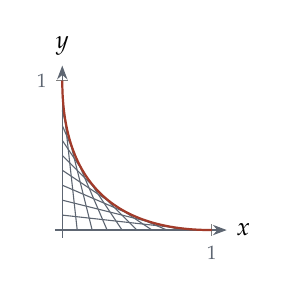
\begin{tikzpicture}
\begin{axis}[courbe,width=0.36\linewidth,xmin=-0.05,xmax=1.1,ymin=-0.05,ymax=1.1,xtick={1},ytick={1}]
\foreach \a in {0.1,0.2,0.3,0.4,0.5,0.6,0.7,0.8,0.9}{\edef\tmp{\noexpand\addplot[Gris,thin] coordinates {(\a,0) (0,{1-\a})};}\tmp}
\addplot[Brique,thick,domain=0:1,samples=60]({x^2},{(1-x)^2});
\end{axis}
\end{tikzpicture}
\end{center}
\piege{élever au carré introduit des points étrangers (la parabole entière contient aussi des points où
$\sqrt x-\sqrt y=\pm1$) : l'enveloppe n'est que l'arc $x,y\in[0,1]$.}
\retenir{droite d'équation $a(t)x+b(t)y=c(t)$ $\Rightarrow$ dériver par rapport au paramètre et résoudre le système $2\times2$.}
\par\hfill\textcolor{BleuClair}{$\square$}\par
\correction{18}{L'hyperbole comme enveloppe}{met-env-hyp}{énoncé : TD, p.~7}
\q{1.} En dérivant par rapport à $t$ : $2ty=2$, d'où $y=\frac1t$, puis $x=2t-t^2\cdot\frac1t=t$. L'enveloppe est paramétrée par $\left(t,\frac1t\right)$, $t\neq0$ : c'est l'hyperbole $xy=1$.

\q{2.} La tangente à $xy=1$ en $\left(t,\frac1t\right)$ a pour pente $-\frac1{t^2}$ (dérivée de $x\mapsto\frac1x$ en $t$) : $y-\frac1t=-\frac{x-t}{t^2}$, soit $t^2y-t=-x+t$, c'est-à-dire $x+t^2y=2t$ : c'est bien $\mathcal D_t$, tangente au point $\left(t,\frac1t\right)$.

\q{3.} $\mathcal D_t$ coupe les axes en $P(2t,0)$ et $Q\left(0,\frac2t\right)$ ; le milieu de $[PQ]$ est $\left(t,\frac1t\right)$. Conséquence : l'aire du triangle $OPQ$ vaut $\frac12\cdot2|t|\cdot\frac2{|t|}=2$, indépendante de $t$.
\par\hfill\textcolor{BleuClair}{$\square$}\par
\partie{III}{Exercices de synthèse et approfondissement}{}
\correction{19}{Repère de Frenet et développée de la cycloïde}{m-cycl-dev}{énoncé : TD, p.~8}
\choix{méthode~1.1 du volume 2 : on écrit $f'=v(\cos\alpha,\sin\alpha)$ grâce à l'angle moitié, et l'on obtient tout d'un coup.}
\q{1.} D'après l'exercice~\ref{e:m-cycl}, $f'=2\sin\frac t2\left(\sin\frac t2,\cos\frac t2\right)$ avec $v=2\sin\frac t2>0$, donc
$\ve T=\left(\sin\frac t2,\cos\frac t2\right)=\left(\cos\alpha,\sin\alpha\right)$ avec $\alpha=\frac\pi2-\frac t2$, et
$\ve N=\left(-\cos\frac t2,\sin\frac t2\right)$. Alors $\gamma=\frac{\alpha'(t)}{v}=\frac{-1/2}{2\sin(t/2)}=-\frac1{4\sin(t/2)}$
($\gamma<0$ : la cycloïde, parcourue de gauche à droite, tourne vers la droite).

\q{2.} $R=-4\sin\frac t2$ et
\begin{align*}
I=M+R\ve N&=(t-\sin t,1-\cos t)+4\sin\tfrac t2\left(\cos\tfrac t2,-\sin\tfrac t2\right)\\
&=\left(t-\sin t+2\sin t,\ 1-\cos t-4\sin^2\tfrac t2\right),
\end{align*}
soit $I=(t+\sin t,\cos t-1)$, car $4\sin^2\frac t2=2(1-\cos t)$.

\q{3.} En posant $t=u+\pi$ : $I=(u-\sin u+\pi,\ -1-\cos u)=(u-\sin u,1-\cos u)+(\pi,-2)$. La développée est la même cycloïde,
translatée de $(\pi,-2)$ : ses rebroussements sont au milieu des arches de la première.
\begin{center}
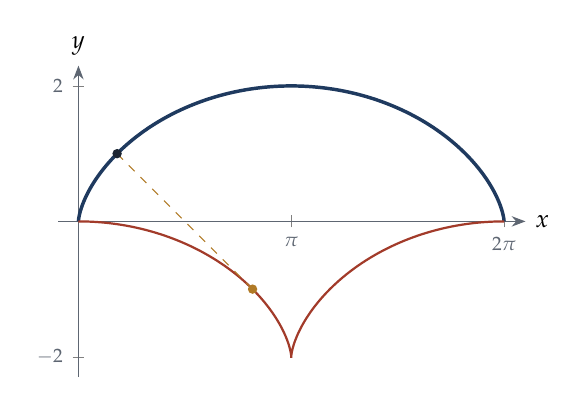
\begin{tikzpicture}
\begin{axis}[courbe,width=0.62\linewidth,xmin=-0.3,xmax=6.6,ymin=-2.3,ymax=2.3,xtick={3.1416,6.2832},xticklabels={$\pi$,$2\pi$},ytick={-2,2}]
\addplot[arcetude,domain=0:6.2832,samples=150]({x-sin(x)},{1-cos(x)});
\addplot[Brique,thick,domain=0:6.2832,samples=150]({x+sin(x)},{cos(x)-1});
\draw[Ocre,dashed] (axis cs:1.5708-1,1)--(axis cs:1.5708+1,-1);
\node[pt] at (axis cs:0.5708,1) {}; \node[pt,fill=Ocre] at (axis cs:2.5708,-1) {};
\end{axis}
\end{tikzpicture}
\end{center}
\retenir{la factorisation par l'angle moitié donne en même temps $v$, $\alpha$, $\ve T$, $\ve N$ ; la développée d'une cycloïde est
une cycloïde (propriété utilisée par Huygens pour le pendule isochrone).}
\par\hfill\textcolor{BleuClair}{$\square$}\par
\correction{20}{Les courbes à courbure constante}{met-courbure-cste}{énoncé : TD, p.~8}
\choix{les formules de Frenet $\frac{d\ve T}{ds}=\gamma\ve N$ et $\frac{d\ve N}{ds}=-\gamma\ve T$ permettent de dériver tout ce qui s'écrit avec $M$, $\ve T$ et $\ve N$.}
\q{1.} $\frac{dI}{ds}=\frac{dM}{ds}+r\frac{d\ve N}{ds}=\ve T-r\gamma\ve T=\ve T-\ve T=\ve0$. Sur l'intervalle de définition, $I$ est donc un point fixe $\Omega$. Alors $\Omega M(s)=\|{-r\ve N(s)}\|=r$ : $\Gamma$ est contenue dans le cercle de centre $\Omega$ et de rayon $r$.

\q{2.} $\frac{d\ve T}{ds}=\gamma\ve N=\ve0$ : $\ve T$ est un vecteur constant $\ve T_0$. Alors $\frac{dM}{ds}=\ve T_0$, donc $M(s)=M(0)+s\,\ve T_0$ : $\Gamma$ est contenue dans la droite passant par $M(0)$ dirigée par $\ve T_0$.
\retenir{courbure constante non nulle : arc de cercle ; courbure nulle : segment de droite. La courbure détermine la forme de la courbe.}
\par\hfill\textcolor{BleuClair}{$\square$}\par
\correction{21}{Courbure et développée de la chaînette}{met-chain-dev}{énoncé : TD, p.~8}
\q{1.} Formule du graphe (exercice~\ref{e:met-graphe}) : $\gamma=\frac{\ch x}{(1+\sh^2x)^{3/2}}=\frac{\ch x}{\ch^3x}=\frac1{\ch^2x}$, donc $R=\ch^2x$.

\q{2.} $f'=(1,\sh x)$, $\|f'\|=\ch x$, $\ve T=\frac{(1,\sh x)}{\ch x}$, $\ve N=\frac{(-\sh x,1)}{\ch x}$. Donc
\[I=M+R\ve N=(x,\ch x)+\ch x\,(-\sh x,1)=\big(x-\sh x\ch x,\ 2\ch x\big).\]

\q{3.} La normale est $M+\lambda\ve N$ ; elle coupe $(Ox)$ quand $\ch x+\frac{\lambda}{\ch x}=0$, c'est-à-dire $\lambda=-\ch^2x$ : $N=M-\ch^2x\,\ve N$. Comme $I=M+\ch^2x\,\ve N$, on a $\vv{MI}=-\vv{MN}$ : $M$ est le milieu de $[IN]$, et $MI=MN=\ch^2x$.
\par\hfill\textcolor{BleuClair}{$\square$}\par
\correction{22}{Développée de l'ellipse comme enveloppe des normales}{e-ellipse}{énoncé : TD, p.~9}
\choix{théorème~2.3 du volume 2 : plutôt que de calculer $R$ et $\ve N$, on enveloppe les normales, ce qui ne demande qu'un
système linéaire.}
\q{1.} La normale passe par $M(t)$ et est orthogonale à $f'(t)=(-a\sin t,b\cos t)$ :
$-a\sin t\,(x-a\cos t)+b\cos t\,(y-b\sin t)=0$, soit
\[ax\sin t-by\cos t=(a^2-b^2)\sin t\cos t.\]
\q{2.} En dérivant par rapport à $t$ : $ax\cos t+by\sin t=(a^2-b^2)\cos2t$. Le système a pour déterminant
$ab(\sin^2t+\cos^2t)=ab\neq0$ ; on obtient
\[x=\frac{a^2-b^2}a\cos^3t,\qquad y=-\frac{a^2-b^2}b\sin^3t.\]
La développée est une astroïde étirée (astroïde de Lamé), avec quatre rebroussements sur les axes.

\q{3.} En $t=0$ : le centre de courbure est $\left(a-\frac{b^2}a,0\right)$, à la distance $\frac{b^2}a$ du sommet $(a,0)$ ; en $t=\frac\pi2$ :
$\left(0,b-\frac{a^2}b\right)$, à la distance $\frac{a^2}b$ de $(0,b)$. Ce sont bien les rayons de courbure trouvés.
\begin{center}
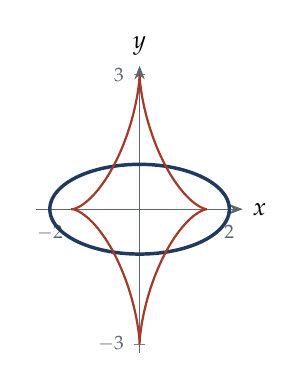
\begin{tikzpicture}
\begin{axis}[courbe,width=0.5\linewidth,xmin=-2.3,xmax=2.3,ymin=-3.2,ymax=3.2,xtick={-2,2},ytick={-3,3}]
\addplot[arcetude,domain=0:6.2832,samples=150]({2*cos(x)},{sin(x)});
\addplot[Brique,thick,domain=0:6.2832,samples=200]({1.5*cos(x)^3},{-3*sin(x)^3});
\end{axis}
\end{tikzpicture}
\end{center}
\gain{les quatre rebroussements de la développée correspondent aux quatre sommets de l'ellipse, où la courbure est
extrémale : c'est le réflexe du chapitre~1.}
\retenir{développée $=$ enveloppe des normales : équation de la normale, dérivée par rapport au paramètre, système $2\times2$.}
\par\hfill\textcolor{BleuClair}{$\square$}\par
\correction{23}{Développée de l'astroïde}{met-astro-dev}{énoncé : TD, p.~9}
\q{1.} $f'(t)=3\sin t\cos t\,(-\cos t,\ \sin t)$ avec $3\sin t\cos t>0$ sur $\left]0,\frac\pi2\right[$. Donc $v=3\sin t\cos t$, $\ve T=(-\cos t,\sin t)$, $\ve N=(-\sin t,-\cos t)$. L'angle $\alpha$ de la tangente vérifie $\ve T=(\cos\alpha,\sin\alpha)$ avec $\alpha=\pi-t$, donc $\frac{d\alpha}{dt}=-1$ et
\[\gamma=\frac{d\alpha}{ds}=\frac{-1}{3\sin t\cos t},\qquad R=-3\sin t\cos t.\]
(Le signe négatif : la courbe tourne dans le sens indirect pour ce sens de parcours.)

\q{2.} $I=M+R\ve N=(\cos^3t,\sin^3t)+3\sin t\cos t\,(\sin t,\cos t)=\big(\cos^3t+3\cos t\sin^2t,\ \sin^3t+3\sin t\cos^2t\big)$. Avec $\sin^2t=\frac{1-\cos2t}2$ : $\cos^3t+3\cos t\sin^2t=\cos t\,(\cos^2t+3\sin^2t)=\cos t\,(2-\cos2t)$, et de même $\sin t\,(\sin^2t+3\cos^2t)=\sin t\,(2+\cos2t)$.

\q{3.} Avec $c=\cos t$, $s=\sin t$ : $u=c^3+3cs^2+3c^2s+s^3=(c+s)^3$ et $v=s^3+3sc^2-c^3-3cs^2=(s-c)^3$. Or $c+s=\sqrt2\cos\left(t-\frac\pi4\right)$ et $s-c=\sqrt2\sin\left(t-\frac\pi4\right)$, donc avec $\tau=t-\frac\pi4$ :
\[u=2\sqrt2\cos^3\tau,\qquad v=2\sqrt2\sin^3\tau.\]
Les coordonnées $(u,v)$ sont celles de $I$, au facteur $\sqrt2$ près, dans le repère orthonormé tourné de $\frac\pi4$ : $\left(\frac u{\sqrt2},\frac v{\sqrt2}\right)=2(\cos^3\tau,\sin^3\tau)$. La développée est donc l'image de l'astroïde par la similitude de centre $O$, de rapport $2$ et d'angle $\frac\pi4$.
\par\hfill\textcolor{BleuClair}{$\square$}\par
\partie{IV}{Exercice difficile et type concours}{}
\correction{24}{Tractrice et chaînette (type concours)}{met-tractrice}{énoncé : TD, p.~10}
\q{1.} $x'=1-\frac1{\ch^2t}=\th^2t$ et $y'=-\frac{\sh t}{\ch^2t}=-\frac{\th t}{\ch t}$. Donc
\[f'(t)=\th t\left(\th t,\ -\frac1{\ch t}\right),\qquad\|f'\|^2=\th^2t\left(\th^2t+\frac1{\ch^2t}\right)=\th^2t,\]
car $\sh^2+1=\ch^2$. Pour $t>0$, $\|f'\|=\th t$ et $s(t)=\int_0^t\th u\,du=\ln\ch t$.

\q{2.} La tangente en $M$ est dirigée par $\ve T=\left(\th t,-\frac1{\ch t}\right)$, \emph{unitaire}. On cherche $\lambda$ tel que $M+\lambda\ve T$ soit sur $(Ox)$ : $\frac1{\ch t}-\frac\lambda{\ch t}=0$, d'où $\lambda=1$ et $P=M+\ve T=(t-\th t+\th t,\ 0)=(t,0)$. Ainsi $MP=\|\ve T\|=1$. Interprétation : un objet $M$ tiré par une laisse de longueur $1$ dont l'extrémité $P$ avance sur $(Ox)$ décrit la tractrice ; la laisse est toujours tangente à la trajectoire.

\q{3.} $\ve N$ s'obtient par rotation de $+\frac\pi2$ : $\ve N=\left(\frac1{\ch t},\ \th t\right)$. L'angle de la tangente vérifie $\cos\alpha=\th t$, $\sin\alpha=-\frac1{\ch t}$. En dérivant $\cos\alpha=\th t$ : $-\sin\alpha\,\alpha'=\frac1{\ch^2t}$, donc $\alpha'=\frac1{\ch t}$, puis
\[\gamma=\frac{d\alpha}{ds}=\frac{\alpha'}{s'}=\frac{1/\ch t}{\th t}=\frac1{\sh t},\qquad R=\sh t.\]
$I=M+R\ve N=\left(t-\th t+\frac{\sh t}{\ch t},\ \frac1{\ch t}+\sh t\,\th t\right)=\left(t,\ \frac{1+\sh^2t}{\ch t}\right)=(t,\ch t)$. La développée de la tractrice est la chaînette $y=\ch x$.

\q{4.} $s=\ln\ch t$ donne $\ch t=e^s$, donc $y=\frac1{\ch t}=e^{-s}$. Et $R=\frac{ds}{d\alpha}=\frac{s'}{\alpha'}=\th t\,\ch t=\sh t=\sqrt{e^{2s}-1}$, ce qui confirme le résultat de la question 3.
\retenir{une courbe dont la tangente unitaire « tombe » toujours sur une droite fixe à distance constante est une tractrice ; sa développée est une chaînette.}
\par\hfill\textcolor{BleuClair}{$\square$}\par
\end{document}
